\documentclass{article}
\usepackage[margin=1in]{geometry}
\usepackage{amsmath}
\usepackage{listings}
\usepackage{color}
\usepackage{graphicx}

\definecolor{dkgreen}{rgb}{0,0.6,0}
\definecolor{gray}{rgb}{0.5,0.5,0.5}
\definecolor{mauve}{rgb}{0.58,0,0.82}

\lstset{frame=tb,
  language=Python,
  aboveskip=3mm,
  belowskip=3mm,
  showstringspaces=false,
  columns=flexible,
  basicstyle={\small\ttfamily},
  numbers=none,
  numberstyle=\tiny\color{gray},
  keywordstyle=\color{blue},
  commentstyle=\color{dkgreen},
  stringstyle=\color{mauve},
  breaklines=true,
  breakatwhitespace=true,
  tabsize=3
}

\begin{document}
\begin{titlepage}
	\setlength{\parindent}{0pt}
	\large

\vspace*{-2cm}

University of Waterloo \par
Econ 424 \par
2023-09-12 \par
\vspace{0.05cm}
Anonymized Usernmae: IJustWannaPass
\vspace{0.2cm}

{\huge Prediction Competition \# 2 \par}
\hrule

\vspace{1cm}
\textbf{Q1)} For our training data we have the following values on our training data (done using a 10-90 split of test vs training), averaged across 100 different runs:
\begin{align*}
R^2 &=  0.73569\\
MSE &= 0.47404
\end{align*}
The hyper parameters of this model where turned by comparing all iterations across 10 different splits of training and test data.\\\\
\textbf{Q2)} The relative importance of the features in the final model can be seen below: \\

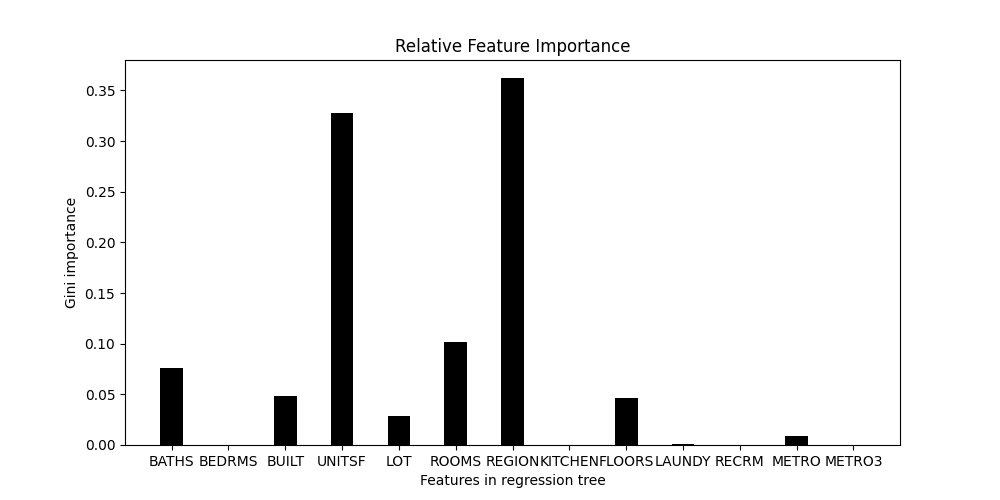
\includegraphics[width=\textwidth]{relativeImportance.png}

Due to the fact that each leaf needs to have ~50 observations alot of features arent used (and thus have zero importance) as the tree is not deep enough to make use of them. \\

\newpage

\textbf{Q3)} To begin with question 1, I asked chatGPT 3.5 the following prompt:


\includegraphics[width=\textwidth]{1.png}
To which chatGPT gave the following response:\\

\begin{center}
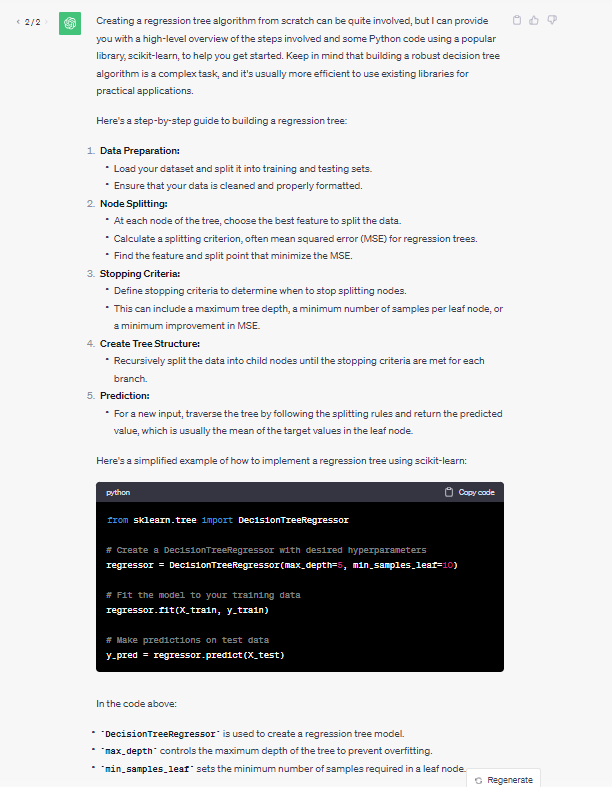
\includegraphics[width=0.8\textwidth]{2.png}
\end{center}
\newpage
As for question 2, I began with the prompt:\\

\includegraphics[width=\textwidth]{3.png}
To which chatGPT replied:\\
\begin{center}
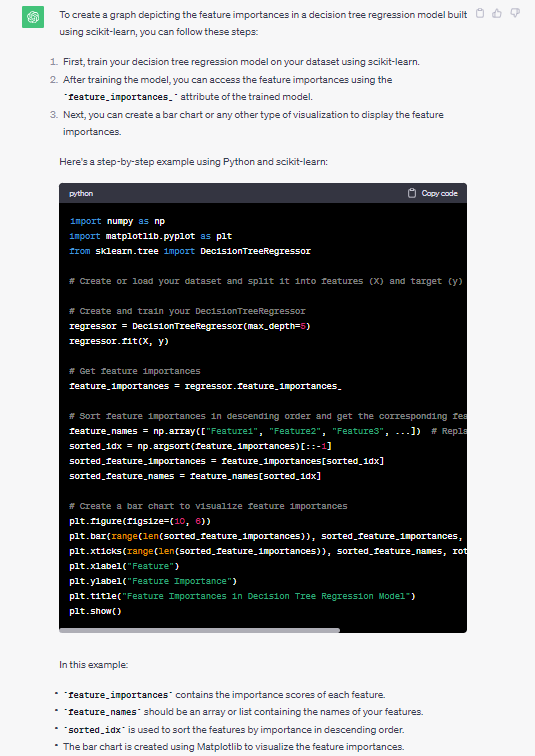
\includegraphics[width=0.8\textwidth]{4.png}
\end{center}


\end{titlepage}

\newpage
\textbf{Code for Q1:}
\begin{lstlisting}
import matplotlib.pyplot as plt
import numpy as np
import pandas as pd
import heapq

from sklearn.tree import DecisionTreeRegressor
from sklearn.model_selection import train_test_split
from scipy import stats

data = pd.read_csv("Econ424_F2023_PC2_training_set_v1.csv", low_memory=False)

# Clean Data
data = data[(np.abs(stats.zscore(data)) < 4).all(axis=1)]

#  =============== PART 1 (Test the model) ===============
X_Train = [0]*100
Y_Train = [0]*100
X_Test = [0]*100
Y_Test = [0]*100

# Load up an array of test and training data

for i in range(0,100):
    train, test = train_test_split(data, test_size=0.1)

    Y_Train[i] = train.iloc[:, 0]
    X_Train[i] = train.iloc[:, 1:]
    Y_Test[i] = test.iloc[:, 0]
    X_Test[i] = test.iloc[:, 1:]

mse = [0]*100
TSS = [0]*100
RSS = [0]*100
regr_1 = DecisionTreeRegressor(max_depth=6, min_samples_leaf=50,min_samples_split=19)
for i in range(0,100):
    regr_1.fit(X_Train[i], Y_Train[i]) # Fit the regression tree with the corresponding values

    predicted_vals = regr_1.predict(X_Test[i])
    r2_mean = np.mean(Y_Test[i].iloc[i])
    for x in range(0, len(predicted_vals)):
        # Calculation for MSE
        mse[i] += ((predicted_vals[x] - Y_Test[i].iloc[x])**2)/len(predicted_vals)
        # Calculation for RSS
        RSS[i] += ((predicted_vals[x] - Y_Test[i].iloc[x])**2)
        TSS[i] += ((r2_mean - Y_Test[i].iloc[x])**2)

print("MSE: " + str(np.mean(mse)))
print("R2: " + str(1-(np.mean(RSS)/np.mean(TSS))))
#  =============== PART 2 (Predict the data) ===============

# Load Data for Prediction In
X_Test = pd.read_csv("Econ424_F2023_PC2_test_set_without_response_variable_v1.csv", low_memory=False)
X_Test.rename(str.upper, axis='columns', inplace=True)

Y_Train = data.iloc[:, 0]
X_Train = data.iloc[:, 1:]

# Train the decision tree with the optimal values
regr_1.fit(X_Train, Y_Train)

estimates = regr_1.predict(X_Test)

# Write the output
f = open('predictions.csv', 'w')
for estimate in estimates:
    f.writelines(str(estimate) + ",\n")
\end{lstlisting}
\newpage

\textbf{Code for Q2:}
\begin{lstlisting}
import matplotlib.pyplot as plt
import numpy as np
import pandas as pd
import heapq

from sklearn.tree import DecisionTreeRegressor
from sklearn.model_selection import train_test_split
from scipy import stats

data = pd.read_csv("Econ424_F2023_PC2_training_set_v1.csv", low_memory=False)

# Clean Data
data = data[(np.abs(stats.zscore(data)) < 4).all(axis=1)]

regr_1 = DecisionTreeRegressor(max_depth=6, min_samples_leaf=50,min_samples_split=19)

Y_Train = data.iloc[:, 0]
X_Train = data.iloc[:, 1:]

X_Test = pd.read_csv("Econ424_F2023_PC2_test_set_without_response_variable_v1.csv", low_memory=False)
X_Test.rename(str.upper, axis='columns', inplace=True)

regr_1.fit(X_Train, Y_Train)


plt.figure(figsize=(10, 5))

plt.bar(regr_1.feature_names_in_, regr_1.feature_importances_, color='black',
        width=0.4)

plt.xlabel("Features in regression tree")
plt.ylabel("Gini importance")
plt.title("Relative Feature Importance")
plt.show()
\end{lstlisting}
\end{document}